\chapter{Evaluation}\label{sec:evaluation}

\section{Software Simulation}

In the LATOME HLS team, the software simulation stack used to validate the firmware is made of 4 layers. Each layer can catch different types of bug, and the higher the layer, the more time it takes to run and the more complex it becomes. Every layer runs automatically when the code is pushed to the repository using Gitlab Continuous Integration (CI).

\subsection{Layer 0}

The layer 0 are divided in two types of tests: the C++ only tests and the RTL tests. The C++ only tests are used to validate the C++ logic used in the HLS blocks. For instance, it can test that an adder function is actually adding two numbers and giving the correct result.

With the same code, also called ``test bench'' the generated RTL files can be tested using Questa simulation. This is very helpful as the test bench code can directly use the C++ HLS types, such as \verb|ac_int| or \verb|ac_channel|. However, the layer 0 has no access to the different clocks and individual signals of the design. For the different blocks, the test bench generates random inputs which are processed with C++ code and compared with the output of the HLS design.

\subsection{Python Test Benches}

\subsubsection{Cocotb}

Layers 1, 2 and 3 use Cocotb, a library which allows to write test benches in Python, and to run them with a simulator, Questa in this case. The Device Under Test (DUT) is the design to be tested, based on the RTL files. The test bench has access to every signal from the DUT, and can monitor them.

These three layers are used to validate the integration of the blocks, and the timing information.

\subsubsection{Firmware Aware and Agnostic Models}

The layers 1, 2 and 3 use a LATOME software model to compare against the RTL outputs. Two models are used to reduce the risk of bugs: the firmware aware model and the firmware agnostic model. The former replicates each blocks of the firmware in Python and gives access to the results at each steps, while the latter is only based on the specifications of the firmware and only gives access to the final outputs.

\subsection{Layer 1}

\begin{figure}[htb]
    \centering
    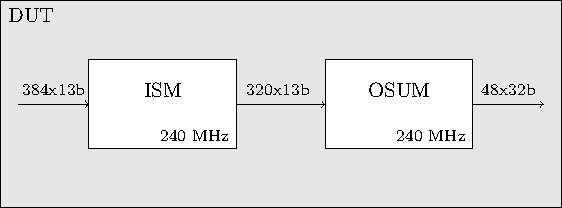
\includegraphics{diagrams/l1}
    \caption{Device Under Test for layer 1}
    \label{fig:dut-l1}
\end{figure}

To only test the HLS code, corresponding to the ISM and the OSUM, the layer 1 uses Python and the Cocotb library, together with Questa simulation. The User Code which connects the ISM and OSUM is a simple bypass at this level. With Cocotb, the test bench can access the different signals of the design, and monitor them. 

This layer uses a simple VHDL wrapper specifically written for it to embed the ISM and OSUM blocks. 

\subsection{Layer 2}

\begin{figure}[htb]
    \centering
    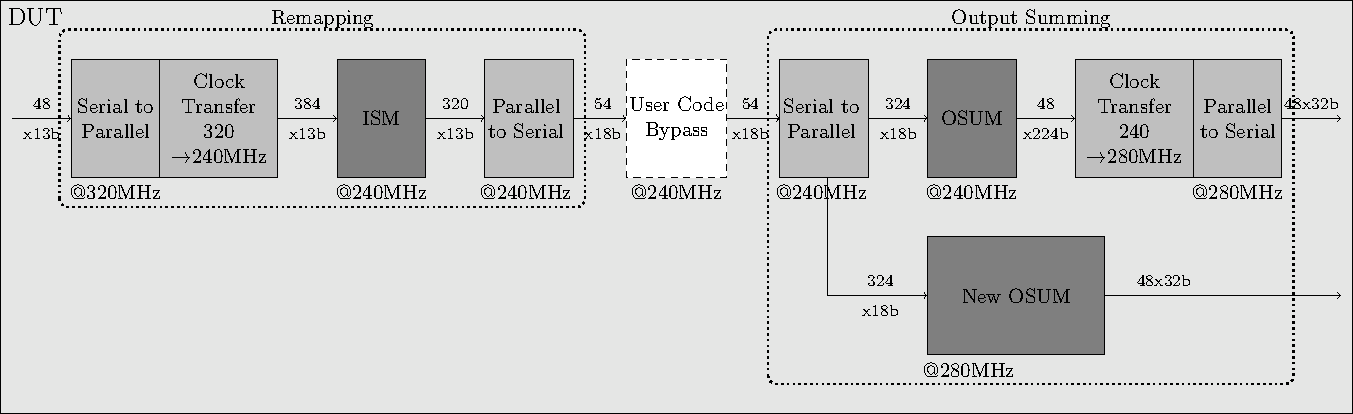
\includegraphics[width=1\textwidth]{diagrams/l2}
    \caption{Device Under Test for layer 2}
    \label{fig:dut-l2}
\end{figure}

The layer 2 tests the RTL files generated by Catapult together with the VHDL code used to convert the serial data to parallel and vice versa, as well as the clock domain transfer blocks. The User Code is still a bypass at this level. 

With the layer 2, the wrapper used, which embeds the HLS blocks and VHDL blocks, is the one used in the final firmware.

\subsection{Layer 3}

The layer 3 is the final layer of the software simulation stack. It tests the whole firmware, including the User Code and software configuration.

\section{Hardware testing}
